\documentclass[12pt,]{book}
\usepackage{lmodern}
\usepackage{amssymb,amsmath}
\usepackage{ifxetex,ifluatex}
\usepackage{fixltx2e} % provides \textsubscript
\ifnum 0\ifxetex 1\fi\ifluatex 1\fi=0 % if pdftex
  \usepackage[T1]{fontenc}
  \usepackage[utf8]{inputenc}
\else % if luatex or xelatex
  \ifxetex
    \usepackage{mathspec}
  \else
    \usepackage{fontspec}
  \fi
  \defaultfontfeatures{Ligatures=TeX,Scale=MatchLowercase}
\fi
% use upquote if available, for straight quotes in verbatim environments
\IfFileExists{upquote.sty}{\usepackage{upquote}}{}
% use microtype if available
\IfFileExists{microtype.sty}{%
\usepackage{microtype}
\UseMicrotypeSet[protrusion]{basicmath} % disable protrusion for tt fonts
}{}
\usepackage{hyperref}
\PassOptionsToPackage{usenames,dvipsnames}{color} % color is loaded by hyperref
\hypersetup{unicode=true,
            pdftitle={Point count data analysis: How to violate assumptions and get away with it},
            pdfauthor={Peter Solymos},
            colorlinks=true,
            linkcolor=Maroon,
            citecolor=Blue,
            urlcolor=Blue,
            breaklinks=true}
\urlstyle{same}  % don't use monospace font for urls
\usepackage{natbib}
\bibliographystyle{apalike}
\usepackage{color}
\usepackage{fancyvrb}
\newcommand{\VerbBar}{|}
\newcommand{\VERB}{\Verb[commandchars=\\\{\}]}
\DefineVerbatimEnvironment{Highlighting}{Verbatim}{commandchars=\\\{\}}
% Add ',fontsize=\small' for more characters per line
\usepackage{framed}
\definecolor{shadecolor}{RGB}{248,248,248}
\newenvironment{Shaded}{\begin{snugshade}}{\end{snugshade}}
\newcommand{\AlertTok}[1]{\textcolor[rgb]{0.94,0.16,0.16}{#1}}
\newcommand{\AnnotationTok}[1]{\textcolor[rgb]{0.56,0.35,0.01}{\textbf{\textit{#1}}}}
\newcommand{\AttributeTok}[1]{\textcolor[rgb]{0.77,0.63,0.00}{#1}}
\newcommand{\BaseNTok}[1]{\textcolor[rgb]{0.00,0.00,0.81}{#1}}
\newcommand{\BuiltInTok}[1]{#1}
\newcommand{\CharTok}[1]{\textcolor[rgb]{0.31,0.60,0.02}{#1}}
\newcommand{\CommentTok}[1]{\textcolor[rgb]{0.56,0.35,0.01}{\textit{#1}}}
\newcommand{\CommentVarTok}[1]{\textcolor[rgb]{0.56,0.35,0.01}{\textbf{\textit{#1}}}}
\newcommand{\ConstantTok}[1]{\textcolor[rgb]{0.00,0.00,0.00}{#1}}
\newcommand{\ControlFlowTok}[1]{\textcolor[rgb]{0.13,0.29,0.53}{\textbf{#1}}}
\newcommand{\DataTypeTok}[1]{\textcolor[rgb]{0.13,0.29,0.53}{#1}}
\newcommand{\DecValTok}[1]{\textcolor[rgb]{0.00,0.00,0.81}{#1}}
\newcommand{\DocumentationTok}[1]{\textcolor[rgb]{0.56,0.35,0.01}{\textbf{\textit{#1}}}}
\newcommand{\ErrorTok}[1]{\textcolor[rgb]{0.64,0.00,0.00}{\textbf{#1}}}
\newcommand{\ExtensionTok}[1]{#1}
\newcommand{\FloatTok}[1]{\textcolor[rgb]{0.00,0.00,0.81}{#1}}
\newcommand{\FunctionTok}[1]{\textcolor[rgb]{0.00,0.00,0.00}{#1}}
\newcommand{\ImportTok}[1]{#1}
\newcommand{\InformationTok}[1]{\textcolor[rgb]{0.56,0.35,0.01}{\textbf{\textit{#1}}}}
\newcommand{\KeywordTok}[1]{\textcolor[rgb]{0.13,0.29,0.53}{\textbf{#1}}}
\newcommand{\NormalTok}[1]{#1}
\newcommand{\OperatorTok}[1]{\textcolor[rgb]{0.81,0.36,0.00}{\textbf{#1}}}
\newcommand{\OtherTok}[1]{\textcolor[rgb]{0.56,0.35,0.01}{#1}}
\newcommand{\PreprocessorTok}[1]{\textcolor[rgb]{0.56,0.35,0.01}{\textit{#1}}}
\newcommand{\RegionMarkerTok}[1]{#1}
\newcommand{\SpecialCharTok}[1]{\textcolor[rgb]{0.00,0.00,0.00}{#1}}
\newcommand{\SpecialStringTok}[1]{\textcolor[rgb]{0.31,0.60,0.02}{#1}}
\newcommand{\StringTok}[1]{\textcolor[rgb]{0.31,0.60,0.02}{#1}}
\newcommand{\VariableTok}[1]{\textcolor[rgb]{0.00,0.00,0.00}{#1}}
\newcommand{\VerbatimStringTok}[1]{\textcolor[rgb]{0.31,0.60,0.02}{#1}}
\newcommand{\WarningTok}[1]{\textcolor[rgb]{0.56,0.35,0.01}{\textbf{\textit{#1}}}}
\usepackage{longtable,booktabs}
\usepackage{graphicx,grffile}
\makeatletter
\def\maxwidth{\ifdim\Gin@nat@width>\linewidth\linewidth\else\Gin@nat@width\fi}
\def\maxheight{\ifdim\Gin@nat@height>\textheight\textheight\else\Gin@nat@height\fi}
\makeatother
% Scale images if necessary, so that they will not overflow the page
% margins by default, and it is still possible to overwrite the defaults
% using explicit options in \includegraphics[width, height, ...]{}
\setkeys{Gin}{width=\maxwidth,height=\maxheight,keepaspectratio}
\IfFileExists{parskip.sty}{%
\usepackage{parskip}
}{% else
\setlength{\parindent}{0pt}
\setlength{\parskip}{6pt plus 2pt minus 1pt}
}
\setlength{\emergencystretch}{3em}  % prevent overfull lines
\providecommand{\tightlist}{%
  \setlength{\itemsep}{0pt}\setlength{\parskip}{0pt}}
\setcounter{secnumdepth}{5}
% Redefines (sub)paragraphs to behave more like sections
\ifx\paragraph\undefined\else
\let\oldparagraph\paragraph
\renewcommand{\paragraph}[1]{\oldparagraph{#1}\mbox{}}
\fi
\ifx\subparagraph\undefined\else
\let\oldsubparagraph\subparagraph
\renewcommand{\subparagraph}[1]{\oldsubparagraph{#1}\mbox{}}
\fi

%%% Use protect on footnotes to avoid problems with footnotes in titles
\let\rmarkdownfootnote\footnote%
\def\footnote{\protect\rmarkdownfootnote}

%%% Change title format to be more compact
\usepackage{titling}

% Create subtitle command for use in maketitle
\providecommand{\subtitle}[1]{
  \posttitle{
    \begin{center}\large#1\end{center}
    }
}

\setlength{\droptitle}{-2em}

  \title{Point count data analysis: How to violate assumptions and get away with it}
    \pretitle{\vspace{\droptitle}\centering\huge}
  \posttitle{\par}
    \author{Peter Solymos}
    \preauthor{\centering\large\emph}
  \postauthor{\par}
      \predate{\centering\large\emph}
  \postdate{\par}
    \date{2019-06-05}

\usepackage{booktabs}
\usepackage{amsthm}
\usepackage[many]{tcolorbox}
\usepackage{graphicx}
\usetikzlibrary{calc}

\makeatletter
\def\thm@space@setup{%
  \thm@preskip=8pt plus 2pt minus 4pt
  \thm@postskip=\thm@preskip
}
\makeatother

% Create our general design
\newtcolorbox{customBlockImage}[2][]{
  enhanced,
  top=10pt,
  bottom=10pt,
  colframe = white,
  width=\textwidth,
  boxsep=5pt,
  arc=1pt,
  outer arc=1pt,
  leftupper=1.5cm,
overlay={
    \node[anchor=west]
      at ([xshift=10pt] $ (interior.north west)!0.5!(interior.south west) $ )
       {{\setkeys{Gin}{width=3em,keepaspectratio}\includegraphics{#2}}};},
#1}

% Define the colours to match the CSS
\definecolor{cexercise}{HTML}{2BBBAD}
\definecolor{cnote}{HTML}{4285F4}
\definecolor{cwarning}{HTML}{AA66CC}

 % Create the new environments for R Markdown
\newenvironment{rmdexercise}
  {\begin{customBlockImage}[colback=cexercise]{images/exercise}}
  {\end{customBlockImage}}

\newenvironment{rmdnote}
  {\begin{customBlockImage}[colback=cnote]{images/note}}
  {\end{customBlockImage}}

\newenvironment{rmdwarning}
  {\begin{customBlockImage}[colback=cwarning]{images/warning}}
  {\end{customBlockImage}}

\urlstyle{tt}

\let\BeginKnitrBlock\begin \let\EndKnitrBlock\end
\begin{document}
\maketitle

{
\hypersetup{linkcolor=black}
\setcounter{tocdepth}{2}
\tableofcontents
}
\listoftables
\listoffigures
\hypertarget{foreword}{%
\chapter*{Foreword}\label{foreword}}
\addcontentsline{toc}{chapter}{Foreword}

This book provides material for the workshop
\emph{Analysis of point-count data in the presence of variable survey methodologies and detection error}
at the \href{https://amornithmeeting.org/}{AOS 2019 conference}
by \href{http://peter.solymos.org}{Peter Solymos}.

The book and related materials in this repository is the basis of a
full day workshop (8 hours long with 3 breaks).

Prior exposure to \href{https://www.r-project.org/}{R} language is necessary
(i.e.~basic R object types and their manipulation, such as arrays, data frames, indexing)
because this is not covered as part of the course.
Check \href{_etc/R-basics.pdf}{this} intro.

\hypertarget{about-the-book-and-the-course}{%
\section{About the book and the course}\label{about-the-book-and-the-course}}

You'll learn

\begin{itemize}
\tightlist
\item
  how to analyze your point count data when it combines different methodologies/protocols/technologies,
\item
  how to violate assumptions and get away with it.
\end{itemize}

\hypertarget{about-the-author}{%
\section{About the author}\label{about-the-author}}

\begin{itemize}
\tightlist
\item
  Ecologist (molluscs, birds),
\item
  pretty good at stats (modeling, detectability, data cloning, multivariate),
\item
  R programmer (vegan, detect, ResourceSelection, pbapply),
\item
  sometimes I teach (like today).
\end{itemize}

\hypertarget{summary-of-course-objectives}{%
\section{Summary of course objectives}\label{summary-of-course-objectives}}

This course is aimed towards ornithologists analyzing field observations,
who are often faced by data heterogeneities due to
field sampling protocols changing from one project to another,
or through time over the lifespan of projects, or trying to combine
`legacy' data sets with new data collected by recording units.
Such heterogeneities can bias analyses when data sets are integrated
inadequately, or can lead to information loss when filtered and standardized to
common standards. Accounting for these issues is important for better
inference regarding status and trend of bird species and communities.

Analysts of such `messy' data sets need to feel comfortable
with manipulating the data, need a full understanding the mechanics of the
models being used (i.e.~critically interpreting the results and acknowledging
assumptions and limitations), and should be able to make informed choices when
faced with methodological challenges.

The course emphasizes critical thinking and active learning.
Participants will be asked to take part in the analysis:
first hand analytics experience from start to finish.
We will use publicly available data sets to demonstrate the data manipulation
and analysis. We will use freely available and open-source R packages.

The expected outcome of the course is a solid foundation for further
professional development via increased confidence in applying these methods
for field observations.

\hypertarget{installing}{%
\section{Installing}\label{installing}}

The \textbf{bookdown} package can be installed from CRAN or Github:

\begin{Shaded}
\begin{Highlighting}[]
\KeywordTok{install.packages}\NormalTok{(}\StringTok{"bookdown"}\NormalTok{)}
\CommentTok{# or the development version}
\CommentTok{# devtools::install_github("rstudio/bookdown")}

\CommentTok{## clean up }
\NormalTok{bookdown}\OperatorTok{::}\KeywordTok{clean_book}\NormalTok{(}\OtherTok{TRUE}\NormalTok{)}
\CommentTok{## rendering the book}
\NormalTok{bookdown}\OperatorTok{::}\KeywordTok{render_book}\NormalTok{(}\StringTok{'index.Rmd'}\NormalTok{, }\StringTok{'bookdown::pdf_book'}\NormalTok{)}
\NormalTok{bookdown}\OperatorTok{::}\KeywordTok{render_book}\NormalTok{(}\StringTok{'index.Rmd'}\NormalTok{, }\StringTok{'bookdown::gitbook'}\NormalTok{)}
\NormalTok{bookdown}\OperatorTok{::}\KeywordTok{render_book}\NormalTok{(}\StringTok{'index.Rmd'}\NormalTok{, }\StringTok{'bookdown::epub_book'}\NormalTok{)}
\end{Highlighting}
\end{Shaded}

To compile this example to PDF, you need XeLaTeX. You are recommended to install TinyTeX (which includes XeLaTeX): \url{https://yihui.name/tinytex/}.

\hypertarget{these-are-just-reminders-to-be-deleted-later}{%
\section{These are just reminders, to be deleted later}\label{these-are-just-reminders-to-be-deleted-later}}

You can label chapter and section titles using \texttt{\{\#label\}} after them, e.g., we can reference Chapter \ref{intro}. If you do not manually label them, there will be automatic labels anyway, e.g., Chapter \ref{methods}.

Figures and tables with captions will be placed in \texttt{figure} and \texttt{table} environments, respectively.

\begin{Shaded}
\begin{Highlighting}[]
\KeywordTok{par}\NormalTok{(}\DataTypeTok{mar =} \KeywordTok{c}\NormalTok{(}\DecValTok{4}\NormalTok{, }\DecValTok{4}\NormalTok{, }\FloatTok{.1}\NormalTok{, }\FloatTok{.1}\NormalTok{))}
\KeywordTok{plot}\NormalTok{(pressure, }\DataTypeTok{type =} \StringTok{'b'}\NormalTok{, }\DataTypeTok{pch =} \DecValTok{19}\NormalTok{)}
\end{Highlighting}
\end{Shaded}

\begin{figure}

{\centering 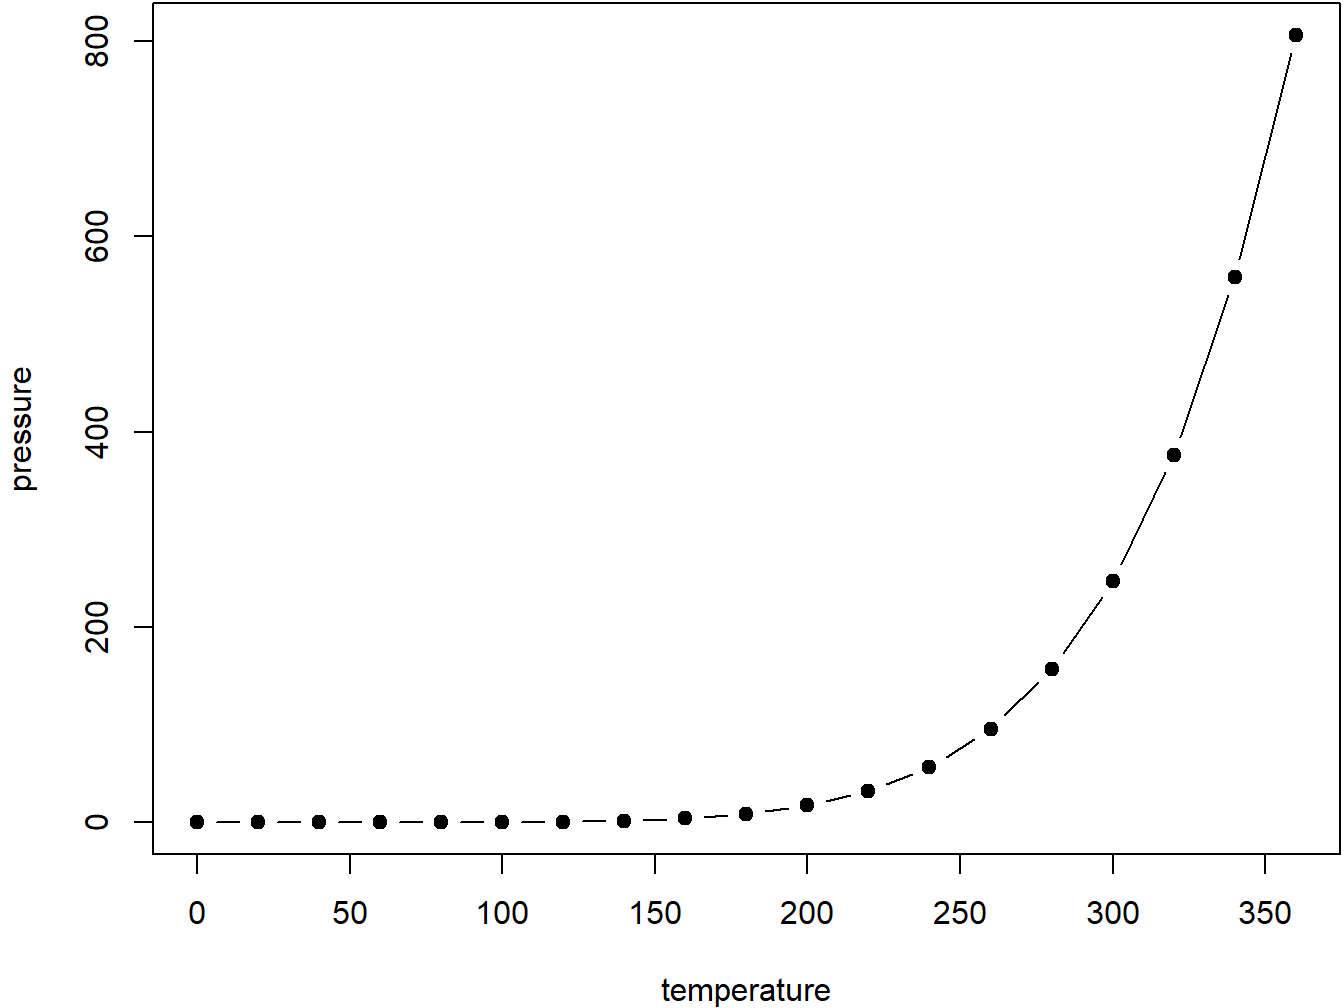
\includegraphics[width=0.8\linewidth]{qpad-book_files/figure-latex/nice-fig-1} 

}

\caption{Here is a nice figure!}\label{fig:nice-fig}
\end{figure}

Reference a figure by its code chunk label with the \texttt{fig:} prefix, e.g., see Figure \ref{fig:nice-fig}. Similarly, you can reference tables generated from \texttt{knitr::kable()}, e.g., see Table \ref{tab:nice-tab}.

\begin{Shaded}
\begin{Highlighting}[]
\NormalTok{knitr}\OperatorTok{::}\KeywordTok{kable}\NormalTok{(}
  \KeywordTok{head}\NormalTok{(iris, }\DecValTok{20}\NormalTok{), }\DataTypeTok{caption =} \StringTok{'Here is a nice table!'}\NormalTok{,}
  \DataTypeTok{booktabs =} \OtherTok{TRUE}
\NormalTok{)}
\end{Highlighting}
\end{Shaded}

\begin{table}[t]

\caption{\label{tab:nice-tab}Here is a nice table!}
\centering
\begin{tabular}{rrrrl}
\toprule
Sepal.Length & Sepal.Width & Petal.Length & Petal.Width & Species\\
\midrule
5.1 & 3.5 & 1.4 & 0.2 & setosa\\
4.9 & 3.0 & 1.4 & 0.2 & setosa\\
4.7 & 3.2 & 1.3 & 0.2 & setosa\\
4.6 & 3.1 & 1.5 & 0.2 & setosa\\
5.0 & 3.6 & 1.4 & 0.2 & setosa\\
\addlinespace
5.4 & 3.9 & 1.7 & 0.4 & setosa\\
4.6 & 3.4 & 1.4 & 0.3 & setosa\\
5.0 & 3.4 & 1.5 & 0.2 & setosa\\
4.4 & 2.9 & 1.4 & 0.2 & setosa\\
4.9 & 3.1 & 1.5 & 0.1 & setosa\\
\addlinespace
5.4 & 3.7 & 1.5 & 0.2 & setosa\\
4.8 & 3.4 & 1.6 & 0.2 & setosa\\
4.8 & 3.0 & 1.4 & 0.1 & setosa\\
4.3 & 3.0 & 1.1 & 0.1 & setosa\\
5.8 & 4.0 & 1.2 & 0.2 & setosa\\
\addlinespace
5.7 & 4.4 & 1.5 & 0.4 & setosa\\
5.4 & 3.9 & 1.3 & 0.4 & setosa\\
5.1 & 3.5 & 1.4 & 0.3 & setosa\\
5.7 & 3.8 & 1.7 & 0.3 & setosa\\
5.1 & 3.8 & 1.5 & 0.3 & setosa\\
\bottomrule
\end{tabular}
\end{table}

You can write citations, too. For example, we are using the \textbf{bookdown} package \citep{R-bookdown} in this sample book, which was built on top of R Markdown and \textbf{knitr} \citep{xie2015}.

\hypertarget{intro}{%
\chapter{Introduction}\label{intro}}

\begin{quote}
All assumptions are violated, but some are more than others
\end{quote}

\hypertarget{apples-and-oranges}{%
\subsubsection{Apples and oranges}\label{apples-and-oranges}}

\emph{``A comparison of apples and oranges occurs when two items or groups of items are compared that
cannot be practically compared.''} {[}\emph{Wikipedia}{]}

How we measure things can have big impact on our results.

\begin{itemize}
\tightlist
\item
  You might say: I saw 5 robins (walking down the road),
\item
  I might say: I only saw one (sitting on my porch)
\end{itemize}

\hypertarget{apples-to-apples}{%
\subsubsection{Apples to apples}\label{apples-to-apples}}

Effort:

\begin{itemize}
\tightlist
\item
  area of the physical space searched,
\item
  amount of time spent,
\item
  number of individuals identified.
\end{itemize}

Experience, skill, ``sensitivity'':

\begin{itemize}
\tightlist
\item
  number of years in field work,
\item
  eye sight, hearing ability,
\item
  mic sensitivity.
\end{itemize}

The goal is to make our measurements comparable.

\hypertarget{effects-can-be-significant}{%
\subsubsection{Effects can be significant}\label{effects-can-be-significant}}

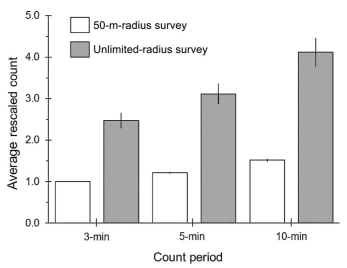
\includegraphics[width=4.82in]{./images/matsuoka-2014-fig-2}

10-min unlimited count \textasciitilde{}300\% increase over 3-min 50-m count.
Average across 54 species of boreal songbirds.

\hypertarget{so-what-is-a-point-count}{%
\subsubsection{So what is a point count?}\label{so-what-is-a-point-count}}

\begin{itemize}
\tightlist
\item
  A trained observer
\item
  records all the birds
\item
  seen and heard
\item
  from a point count station
\item
  for a set period of time
\item
  within a defined distance radius.
\end{itemize}

\hypertarget{questions-we-want-to-answer-using-point-counts}{%
\subsubsection{Questions we want to answer using point counts}\label{questions-we-want-to-answer-using-point-counts}}

\begin{itemize}
\tightlist
\item
  How many? (Abundance, density, population size)
\item
  Is this location part of the range? (0/1)
\item
  How is abundance changing in space? (Distribution)
\item
  How is abundance changing in time? (Trend)
\item
  What is the effect of a treatment on abundance?
\end{itemize}

\hypertarget{standardization-by-design}{%
\subsubsection{Standardization by design}\label{standardization-by-design}}

Have a set of standards/recommendations that people will follow to

\begin{itemize}
\tightlist
\item
  maximize efficiency in the numbers of birds and species counted,
\item
  minimize extraneous variability in the counts.
\end{itemize}

But programs started to deviate from standards:

\emph{``For example, only 3\% of 196,000 point counts conducted during the period
1992--2011 across Alaska and Canada followed the standards recommended for the count period and count radius.''}

\hypertarget{protocols-do-vary}{%
\subsubsection{Protocols do vary}\label{protocols-do-vary}}

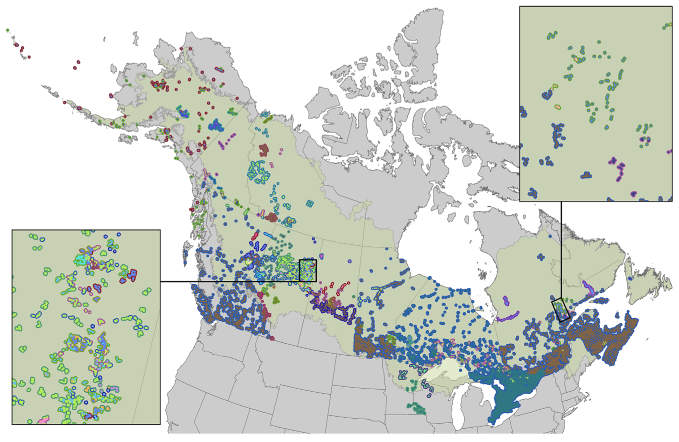
\includegraphics[width=9.43in]{./images/barker-2015-fig-2}

Survey methodology variation (colors) among contributed projects
in the Boreal Avian Modelling (BAM) data base as of 2014.

\BeginKnitrBlock{rmdexercise}
\textbf{Exercise}

In what regard can protocols differ?

What drives protocol variation among projects?

Why have we abandoned following protocols?
\EndKnitrBlock{rmdexercise}

\hypertarget{moving-away-from-standards}{%
\subsubsection{Moving away from standards}\label{moving-away-from-standards}}

\begin{itemize}
\tightlist
\item
  Detection probabilities might vary even with fixed effort (we'll cover this more later),
\item
  programs might have their own goals and constraints (access, training, etc).
\end{itemize}

\hypertarget{model-based-approaches}{%
\subsubsection{Model based approaches}\label{model-based-approaches}}

Less labour intensive methods for unmarked populations has come to the forefront:

\begin{itemize}
\tightlist
\item
  double observer (\href{https://doi.org/10.1642/0004-8038(2000)117\%5B0393:ADOAFE\%5D2.0.CO;2}{Nichols et al.~2000}),
\item
  distance sampling (\href{https://global.oup.com/academic/product/introduction-to-distance-sampling-9780198509271}{Buckland et al.~2001}),
\item
  removal sampling (\href{https://doi.org/10.1642/0004-8038(2002)119\%5B0414:ARMFED\%5D2.0.CO;2}{Farnsworth et al.~2002}),
\item
  multiple visit occupancy (\href{https://doi.org/10.1890/0012-9658(2002)083\%5B2248:ESORWD\%5D2.0.CO;2}{MacKenzie et al.~2002}),
\item
  multiple visit abundance (\href{https://doi.org/10.1111/j.0006-341X.2004.00142.x}{Royle 2004}).
\end{itemize}

\hypertarget{models-come-with-assumptions}{%
\subsubsection{Models come with assumptions}\label{models-come-with-assumptions}}

\begin{itemize}
\tightlist
\item
  Population is closed during multiple visits,
\item
  observers are independent,
\item
  all individuals emit cues with identical rates,
\item
  spatial distribution of individuals is uniform,
\item
  etc. (we will investigate this further in depth).
\end{itemize}

\hypertarget{assumptions-are-everywhere}{%
\subsubsection{Assumptions are everywhere}\label{assumptions-are-everywhere}}

Although assumptions are everywhere, we are really good at ignoring them:

\begin{itemize}
\tightlist
\item
  Relativistic time dilation is negligible (as long as we are not on a space station),
\item
  samples are independent.
\end{itemize}

\BeginKnitrBlock{rmdexercise}
\textbf{Exercise}

Can you mention some other common assumptions?

Can you explain why we neglect/violate assumptions?
\EndKnitrBlock{rmdexercise}

\hypertarget{the-hard-truth}{%
\subsubsection{The hard truth}\label{the-hard-truth}}

Assumptions are violated in many ways, because we seek simplicity.

The main question we have to ask: \textbf{does it matter in practice}?

\hypertarget{our-approach}{%
\subsubsection{Our approach}\label{our-approach}}

\begin{enumerate}
\def\labelenumi{\arabic{enumi}.}
\tightlist
\item
  We will introduce a concept,
\item
  understand how we can infer it from data,
\item
  then we recreate the situation \emph{in silico},
\item
  and see how the outcome changes as we make different assumptions.
\end{enumerate}

It is guaranteed that we violate \textbf{every} assumption we make.

To get away with it, we need to understand \textbf{how much is too much}.

\emph{``All assumptions are violated, but some are more than others.''}

\hypertarget{pcdata}{%
\chapter{Organizing and Processing Point Count Data}\label{pcdata}}

\begin{quote}
All data are messy, but some are missing
\end{quote}

It is often called \emph{data processing}, \emph{data munging},
\emph{data wrangling}, \emph{data cleaning}.
None of these expressions capture the dread associated with the actual activity.

Luckily, there are only 4 things that can get messed up:

\begin{enumerate}
\def\labelenumi{\arabic{enumi}.}
\tightlist
\item
  space (e.g.~wrong UTM zones),
\item
  time (ISO format please),
\item
  taxonomy (UNK, mis-ID),
\item
  something else (if there were no errors, check again).
\end{enumerate}

\hypertarget{josm-joint-oil-sands-monitoring-data}{%
\section{JOSM (Joint Oil Sands Monitoring) data}\label{josm-joint-oil-sands-monitoring-data}}

Look at the source code in the \texttt{\_data/josm} directory of the book
if you are interested in data processing details.
We skip that for now.

\includegraphics[width=13.89in]{./images/mahon-2016-fig-1}

Cause-Effect Monitoring Migratory Landbirds at Regional Scales:
understand how boreal songbirds are affected by human activity in the oil sands area.

\includegraphics[width=13.89in]{./images/mahon-2016-fig-2}

Survey area boundary (\(r\)=2.5 km circle), habitat type and human footprint mapping,
and clustered point count site locations.

Surveys were spatially replicated because:

\begin{itemize}
\tightlist
\item
  we want to make inferences about a population,
\item
  full census is out of reach,
\item
  thus we take a sample of the population
\item
  that is representative and random.
\item
  Ideally, sample size should be as large as possible,
\item
  it reduces variability and
\item
  increases statistical power.
\end{itemize}

Survey locations were pucked based on various criteria:

\begin{itemize}
\tightlist
\item
  stratification (land cover),
\item
  gradients (disturbance levels),
\item
  random location (control for unmeasured effects),
\item
  take into account historical surveys (avoid, or revisit),
\item
  access, cost (clusters).
\end{itemize}

The \texttt{josm} obejct is a list with 3 elements:

\begin{itemize}
\tightlist
\item
  \texttt{surveys}: data frame with survey specific information,
\item
  \texttt{species}: lookup table for species,
\item
  \texttt{counts}: individual counts by survey and species.
\end{itemize}

\begin{Shaded}
\begin{Highlighting}[]
\KeywordTok{library}\NormalTok{(mefa4)}
\KeywordTok{load}\NormalTok{(}\StringTok{"./_data/josm/josm.rda"}\NormalTok{)}
\KeywordTok{names}\NormalTok{(josm)}
\end{Highlighting}
\end{Shaded}

\begin{verbatim}
## [1] "surveys" "species" "counts"
\end{verbatim}

Species info: species codes, common and scientific names. The table could also contain
taxonomic, trait, etc. information as well.

\begin{Shaded}
\begin{Highlighting}[]
\KeywordTok{head}\NormalTok{(josm}\OperatorTok{$}\NormalTok{species)}
\end{Highlighting}
\end{Shaded}

\begin{verbatim}
##      SpeciesID        SpeciesName        ScientificName
## ALFL      ALFL   Alder Flycatcher     Empidonax alnorum
## AMBI      AMBI   American Bittern Botaurus lentiginosus
## AMCO      AMCO      American Coot      Fulica americana
## AMCR      AMCR      American Crow Corvus brachyrhynchos
## AMGO      AMGO American Goldfinch     Carduelis tristis
## AMKE      AMKE   American Kestrel      Falco sparverius
\end{verbatim}

At the survey level, we have coordinates, date/time info,
variables capturing survey conditions, and land cover info extracted from 1 km\(^2\) resolution rasters.

\begin{Shaded}
\begin{Highlighting}[]
\KeywordTok{colnames}\NormalTok{(josm}\OperatorTok{$}\NormalTok{surveys)}
\end{Highlighting}
\end{Shaded}

\begin{verbatim}
##  [1] "SiteID"        "SurveyArea"    "Longitude"    
##  [4] "Latitude"      "Date"          "StationID"    
##  [7] "ObserverID"    "TimeStart"     "VisitID"      
## [10] "WindStart"     "PrecipStart"   "TempStart"    
## [13] "CloudStart"    "WindEnd"       "PrecipEnd"    
## [16] "TempEnd"       "CloudEnd"      "TimeFin"      
## [19] "Noise"         "OvernightRain" "DateTime"     
## [22] "SunRiseTime"   "SunRiseFrac"   "TSSR"         
## [25] "OrdinalDay"    "DAY"           "Open"         
## [28] "Water"         "Agr"           "UrbInd"       
## [31] "SoftLin"       "Roads"         "Decid"        
## [34] "OpenWet"       "Conif"         "ConifWet"
\end{verbatim}

The count table contains one row for each unique individual
of a species (\texttt{SpeciesID} links to the species lookup table)
observed during a survey (\texttt{StationID} links to the survey attribute table).
Check the data dictionary in \texttt{\_data/josm} folder for a detailed explanation of each column.

\begin{Shaded}
\begin{Highlighting}[]
\KeywordTok{str}\NormalTok{(josm}\OperatorTok{$}\NormalTok{counts)}
\end{Highlighting}
\end{Shaded}

\begin{verbatim}
## 'data.frame':    52372 obs. of  18 variables:
##  $ ObservationID: Factor w/ 57024 levels "CL10102-130622-001",..: 1 2 3 4 5 6 8 9 10 11 ...
##  $ SiteID       : Factor w/ 4569 levels "CL10102","CL10106",..: 1 1 1 1 1 1 1 1 2 2 ...
##  $ StationID    : Factor w/ 4569 levels "CL10102-1","CL10106-1",..: 1 1 1 1 1 1 1 1 2 2 ...
##  $ TimeInterval : int  1 1 1 1 5 5 1 1 1 1 ...
##  $ Direction    : int  1 2 2 2 1 4 4 4 1 1 ...
##  $ Distance     : int  1 2 2 1 3 3 2 1 1 1 ...
##  $ DetectType1  : Factor w/ 3 levels "C","S","V": 2 2 2 2 1 1 2 2 2 2 ...
##  $ DetectType2  : Factor w/ 3 levels "C","S","V": NA NA NA NA NA NA NA NA NA NA ...
##  $ DetectType3  : Factor w/ 3 levels "C","S","V": NA NA NA NA NA NA NA NA NA NA ...
##  $ Sex          : Factor w/ 4 levels "F","M","P","U": 2 2 2 2 4 4 2 2 2 2 ...
##  $ Age          : Factor w/ 6 levels "A","F","J","JUV",..: 1 1 1 1 1 1 1 1 1 1 ...
##  $ Activity1    : Factor w/ 17 levels "BE","CF","CH",..: 5 5 5 5 NA NA NA 5 5 NA ...
##  $ Activity2    : Factor w/ 17 levels "48","BE","CF",..: NA NA NA NA NA NA NA NA NA NA ...
##  $ Activity3    : Factor w/ 7 levels "CF","DC","DR",..: NA NA NA NA NA NA NA NA NA NA ...
##  $ ActivityNote : Factor w/ 959 levels "AGITATED","AGITATED CALLING",..: NA NA NA NA NA NA NA NA NA NA ...
##  $ Dur          : Factor w/ 3 levels "0-3min","3-5min",..: 1 1 1 1 3 3 1 1 1 1 ...
##  $ Dis          : Factor w/ 3 levels "0-50m","50-100min",..: 1 2 2 1 3 3 2 1 1 1 ...
##  $ SpeciesID    : Factor w/ 150 levels "ALFL","AMBI",..: 107 95 95 107 46 43 140 95 125 38 ...
\end{verbatim}

\hypertarget{cross-tabulating-species-counts}{%
\section{Cross tabulating species counts}\label{cross-tabulating-species-counts}}

Take the following dummy data frame (long format):

\begin{Shaded}
\begin{Highlighting}[]
\NormalTok{(d <-}\StringTok{ }\KeywordTok{data.frame}\NormalTok{(}
  \DataTypeTok{sample=}\KeywordTok{factor}\NormalTok{(}\KeywordTok{paste0}\NormalTok{(}\StringTok{"S"}\NormalTok{, }\KeywordTok{c}\NormalTok{(}\DecValTok{1}\NormalTok{,}\DecValTok{1}\NormalTok{,}\DecValTok{1}\NormalTok{,}\DecValTok{2}\NormalTok{,}\DecValTok{2}\NormalTok{)), }\KeywordTok{paste0}\NormalTok{(}\StringTok{"S"}\NormalTok{, }\DecValTok{1}\OperatorTok{:}\DecValTok{3}\NormalTok{)),}
  \DataTypeTok{species=}\KeywordTok{c}\NormalTok{(}\StringTok{"BTNW"}\NormalTok{, }\StringTok{"OVEN"}\NormalTok{, }\StringTok{"CANG"}\NormalTok{, }\StringTok{"AMRO"}\NormalTok{, }\StringTok{"CANG"}\NormalTok{),}
  \DataTypeTok{abundance=}\KeywordTok{c}\NormalTok{(}\DecValTok{1}\NormalTok{, }\DecValTok{1}\NormalTok{, }\DecValTok{2}\NormalTok{, }\DecValTok{1}\NormalTok{, }\DecValTok{1}\NormalTok{),}
  \DataTypeTok{behavior=}\KeywordTok{rep}\NormalTok{(}\KeywordTok{c}\NormalTok{(}\StringTok{"heard"}\NormalTok{,}\StringTok{"seen"}\NormalTok{), }\KeywordTok{c}\NormalTok{(}\DecValTok{4}\NormalTok{, }\DecValTok{1}\NormalTok{))))}
\end{Highlighting}
\end{Shaded}

\begin{verbatim}
##   sample species abundance behavior
## 1     S1    BTNW         1    heard
## 2     S1    OVEN         1    heard
## 3     S1    CANG         2    heard
## 4     S2    AMRO         1    heard
## 5     S2    CANG         1     seen
\end{verbatim}

\begin{Shaded}
\begin{Highlighting}[]
\KeywordTok{str}\NormalTok{(d)}
\end{Highlighting}
\end{Shaded}

\begin{verbatim}
## 'data.frame':    5 obs. of  4 variables:
##  $ sample   : Factor w/ 3 levels "S1","S2","S3": 1 1 1 2 2
##  $ species  : Factor w/ 4 levels "AMRO","BTNW",..: 2 4 3 1 3
##  $ abundance: num  1 1 2 1 1
##  $ behavior : Factor w/ 2 levels "heard","seen": 1 1 1 1 2
\end{verbatim}

We want to add up the \texttt{abundance}s for each sample (rows) and species (column):

\begin{Shaded}
\begin{Highlighting}[]
\NormalTok{(y <-}\StringTok{ }\KeywordTok{Xtab}\NormalTok{(abundance }\OperatorTok{~}\StringTok{ }\NormalTok{sample }\OperatorTok{+}\StringTok{ }\NormalTok{species, d))}
\end{Highlighting}
\end{Shaded}

\begin{verbatim}
## 3 x 4 sparse Matrix of class "dgCMatrix"
##    AMRO BTNW CANG OVEN
## S1    .    1    2    1
## S2    1    .    1    .
## S3    .    .    .    .
\end{verbatim}

\texttt{y} is a sparse matrix, that is a very compact representation:

\begin{Shaded}
\begin{Highlighting}[]
\KeywordTok{object.size}\NormalTok{(d[,}\DecValTok{1}\OperatorTok{:}\DecValTok{3}\NormalTok{])}
\end{Highlighting}
\end{Shaded}

\begin{verbatim}
## 2328 bytes
\end{verbatim}

\begin{Shaded}
\begin{Highlighting}[]
\KeywordTok{object.size}\NormalTok{(y)}
\end{Highlighting}
\end{Shaded}

\begin{verbatim}
## 2160 bytes
\end{verbatim}

Notice that we have 3 rows, but \texttt{d\$sample} did not have an \texttt{S3} value, but it was a level.
We can drop such unused levels, but it is generally not recommended, and we need to be careful
not to drop samples where no species was detected (this can happen quite often depending on timing of
surveys)

\begin{Shaded}
\begin{Highlighting}[]
\KeywordTok{Xtab}\NormalTok{(abundance }\OperatorTok{~}\StringTok{ }\NormalTok{sample }\OperatorTok{+}\StringTok{ }\NormalTok{species, d, }\DataTypeTok{drop.unused.levels =} \OtherTok{TRUE}\NormalTok{)}
\end{Highlighting}
\end{Shaded}

\begin{verbatim}
## 2 x 4 sparse Matrix of class "dgCMatrix"
##    AMRO BTNW CANG OVEN
## S1    .    1    2    1
## S2    1    .    1    .
\end{verbatim}

A sparse matrix can be converted to ordinary matrix

\begin{Shaded}
\begin{Highlighting}[]
\KeywordTok{as.matrix}\NormalTok{(y)}
\end{Highlighting}
\end{Shaded}

\begin{verbatim}
##    AMRO BTNW CANG OVEN
## S1    0    1    2    1
## S2    1    0    1    0
## S3    0    0    0    0
\end{verbatim}

The nice thing about this cross tabulation is that we can finter the records without
changing the structure (rows, columns) of the table:

\begin{Shaded}
\begin{Highlighting}[]
\KeywordTok{Xtab}\NormalTok{(abundance }\OperatorTok{~}\StringTok{ }\NormalTok{sample }\OperatorTok{+}\StringTok{ }\NormalTok{species, d[d}\OperatorTok{$}\NormalTok{behavior }\OperatorTok{==}\StringTok{ "heard"}\NormalTok{,])}
\end{Highlighting}
\end{Shaded}

\begin{verbatim}
## 3 x 4 sparse Matrix of class "dgCMatrix"
##    AMRO BTNW CANG OVEN
## S1    .    1    2    1
## S2    1    .    .    .
## S3    .    .    .    .
\end{verbatim}

\begin{Shaded}
\begin{Highlighting}[]
\KeywordTok{Xtab}\NormalTok{(abundance }\OperatorTok{~}\StringTok{ }\NormalTok{sample }\OperatorTok{+}\StringTok{ }\NormalTok{species, d[d}\OperatorTok{$}\NormalTok{behavior }\OperatorTok{==}\StringTok{ "seen"}\NormalTok{,])}
\end{Highlighting}
\end{Shaded}

\begin{verbatim}
## 3 x 4 sparse Matrix of class "dgCMatrix"
##    AMRO BTNW CANG OVEN
## S1    .    .    .    .
## S2    .    .    1    .
## S3    .    .    .    .
\end{verbatim}

Now let's do this for the real data. We have no abundance column, because
each row stands for exactly one individual. We can add a column with 1's,
or we can just count the number of rows by using only the right-hand-side of the
formula in \texttt{Xtab}. \texttt{ytot} will be our total count matrix for now.

We also want to filter the records to contain only \texttt{S}ongs and \texttt{C}alls, without
\texttt{V}visual detections:

\begin{Shaded}
\begin{Highlighting}[]
\KeywordTok{table}\NormalTok{(josm}\OperatorTok{$}\NormalTok{counts}\OperatorTok{$}\NormalTok{DetectType1, }\DataTypeTok{useNA=}\StringTok{"always"}\NormalTok{)}
\end{Highlighting}
\end{Shaded}

\begin{verbatim}
## 
##     C     S     V  <NA> 
##  9180 41808  1384     0
\end{verbatim}

We use \texttt{SiteID} for row names, because only 1 station and visit was done at each site:

\begin{Shaded}
\begin{Highlighting}[]
\NormalTok{ytot <-}\StringTok{ }\KeywordTok{Xtab}\NormalTok{(}\OperatorTok{~}\StringTok{ }\NormalTok{SiteID }\OperatorTok{+}\StringTok{ }\NormalTok{SpeciesID , josm}\OperatorTok{$}\NormalTok{counts[josm}\OperatorTok{$}\NormalTok{counts}\OperatorTok{$}\NormalTok{DetectType1 }\OperatorTok{!=}\StringTok{ "V"}\NormalTok{,])}
\end{Highlighting}
\end{Shaded}

See how not storing 0's affect size compared to the long formar and an ordinary wide matrix

\begin{Shaded}
\begin{Highlighting}[]
\CommentTok{## 2-column data frame as reference}
\NormalTok{tmp <-}\StringTok{ }\KeywordTok{as.numeric}\NormalTok{(}\KeywordTok{object.size}\NormalTok{(}
\NormalTok{  josm}\OperatorTok{$}\NormalTok{counts[josm}\OperatorTok{$}\NormalTok{counts}\OperatorTok{$}\NormalTok{DetectType1 }\OperatorTok{!=}\StringTok{ "V"}\NormalTok{, }\KeywordTok{c}\NormalTok{(}\StringTok{"StationID"}\NormalTok{, }\StringTok{"SpeciesID"}\NormalTok{)]))}
\CommentTok{## spare matrix}
\KeywordTok{as.numeric}\NormalTok{(}\KeywordTok{object.size}\NormalTok{(ytot)) }\OperatorTok{/}\StringTok{ }\NormalTok{tmp}
\end{Highlighting}
\end{Shaded}

\begin{verbatim}
## [1] 0.1366
\end{verbatim}

\begin{Shaded}
\begin{Highlighting}[]
\CommentTok{## dense matrix}
\KeywordTok{as.numeric}\NormalTok{(}\KeywordTok{object.size}\NormalTok{(}\KeywordTok{as.matrix}\NormalTok{(ytot))) }\OperatorTok{/}\StringTok{ }\NormalTok{tmp}
\end{Highlighting}
\end{Shaded}

\begin{verbatim}
## [1] 1.106
\end{verbatim}

\begin{Shaded}
\begin{Highlighting}[]
\CommentTok{## matrix fill}
\KeywordTok{sum}\NormalTok{(ytot }\OperatorTok{>}\StringTok{ }\DecValTok{0}\NormalTok{) }\OperatorTok{/}\StringTok{ }\KeywordTok{prod}\NormalTok{(}\KeywordTok{dim}\NormalTok{(ytot))}
\end{Highlighting}
\end{Shaded}

\begin{verbatim}
## [1] 0.04911
\end{verbatim}

Check if counts are as expected:

\begin{Shaded}
\begin{Highlighting}[]
\KeywordTok{max}\NormalTok{(ytot) }\CommentTok{# this is interesting}
\end{Highlighting}
\end{Shaded}

\begin{verbatim}
## [1] 200
\end{verbatim}

\begin{Shaded}
\begin{Highlighting}[]
\KeywordTok{sort}\NormalTok{(}\KeywordTok{apply}\NormalTok{(}\KeywordTok{as.matrix}\NormalTok{(ytot), }\DecValTok{2}\NormalTok{, max)) }\CommentTok{# it is CANG}
\end{Highlighting}
\end{Shaded}

\begin{verbatim}
## BUFF BWTE COGO COHA DCCO GWTE HOLA NHOW NSHO RTHU WWSC CANV NOPI 
##    0    0    0    0    0    0    0    0    0    0    0    0    0 
## AMBI AMCO AMGO BAEA BAOR BEKI BOWA CONI CSWA EAPH GBHE GCTH GGOW 
##    1    1    1    1    1    1    1    1    1    1    1    1    1 
## GHOW HOWR LEOW MERL NESP NOGO NOHA NSWO PBGR RBGU RTHA SAVS SPSA 
##    1    1    1    1    1    1    1    1    1    1    1    1    1 
## WBNU BRBL CAGU MYWA SNBU VEER AMKE AMWI BADO BARS BBWO BHCO BLBW 
##    1    1    1    1    1    1    2    2    2    2    2    2    2 
## BLPW BLTE BWHA COGR DOWO EAKI HAWO KILL LEYE NAWA NOPO OSFL OSPR 
##    2    2    2    2    2    2    2    2    2    2    2    2    2 
## PIWO PUFI RNDU SORA SSHA COSN AMCR AMRO ATTW BHVI BOCH BRCR BTNW 
##    2    2    2    2    2    2    3    3    3    3    3    3    3 
## CMWA FOSP FRGU GCKI MAWR MOWA NOFL PHVI SACR SOSA SOSP SPGR TRES 
##    3    3    3    3    3    3    3    3    3    3    3    3    3 
## WETA WIWA WIWR YBSA FOTE BAWW BBWA BCCH BLJA CAWA CONW COTE GRYE 
##    3    3    3    3    3    4    4    4    4    4    4    4    4 
## NOWA NRWS OCWA REVI RNGR RUBL RWBL WAVI WEWP WISN YBFL YWAR ALFL 
##    4    4    4    4    4    4    4    4    4    4    4    4    5 
## AMRE CHSP CORA EVGR HETH LCSP RBGR RBNU RCKI SWSP CCSP COYE DEJU 
##    5    5    5    5    5    5    5    5    5    5    6    6    6 
## LEFL LISP MAWA OVEN RUGR SWTH BOGU MALL GRAJ PAWA WTSP YRWA COLO 
##    6    6    6    6    6    6    7    7    8    8    8    8    9 
## TEWA AMPI WWCR CEDW PISI RECR CANG 
##   12   12   20   23   50   51  200
\end{verbatim}

\begin{Shaded}
\begin{Highlighting}[]
\CommentTok{## lyover (FO) flock (FL) beyond 100m distance}
\KeywordTok{head}\NormalTok{(josm}\OperatorTok{$}\NormalTok{counts[}
\NormalTok{  josm}\OperatorTok{$}\NormalTok{counts}\OperatorTok{$}\NormalTok{SiteID }\OperatorTok{==}\StringTok{ }\KeywordTok{rownames}\NormalTok{(ytot)[}\KeywordTok{which}\NormalTok{(ytot[,}\StringTok{"CANG"}\NormalTok{] }\OperatorTok{==}\StringTok{ }\DecValTok{200}\NormalTok{)] }\OperatorTok{&}
\StringTok{  }\NormalTok{josm}\OperatorTok{$}\NormalTok{counts}\OperatorTok{$}\NormalTok{SpeciesID }\OperatorTok{==}\StringTok{ "CANG"}\NormalTok{,])}
\end{Highlighting}
\end{Shaded}

\begin{verbatim}
##                         ObservationID  SiteID StationID
## CO10712-130603-008 CO10712-130603-008 CO10712 CO10712-1
## CO10712-130603-009 CO10712-130603-009 CO10712 CO10712-1
## CO10712-130603-010 CO10712-130603-010 CO10712 CO10712-1
## CO10712-130603-011 CO10712-130603-011 CO10712 CO10712-1
## CO10712-130603-012 CO10712-130603-012 CO10712 CO10712-1
## CO10712-130603-013 CO10712-130603-013 CO10712 CO10712-1
##                    TimeInterval Direction Distance DetectType1
## CO10712-130603-008            1         2        3           C
## CO10712-130603-009            1         2        3           C
## CO10712-130603-010            1         2        3           C
## CO10712-130603-011            1         2        3           C
## CO10712-130603-012            1         2        3           C
## CO10712-130603-013            1         2        3           C
##                    DetectType2 DetectType3 Sex Age Activity1
## CO10712-130603-008        <NA>        <NA>   U   A        FO
## CO10712-130603-009        <NA>        <NA>   U   A        FO
## CO10712-130603-010        <NA>        <NA>   U   A        FO
## CO10712-130603-011        <NA>        <NA>   U   A        FO
## CO10712-130603-012        <NA>        <NA>   U   A        FO
## CO10712-130603-013        <NA>        <NA>   U   A        FO
##                    Activity2 Activity3 ActivityNote    Dur   Dis
## CO10712-130603-008        FL      <NA>         <NA> 0-3min 100+m
## CO10712-130603-009        FL      <NA>         <NA> 0-3min 100+m
## CO10712-130603-010        FL      <NA>         <NA> 0-3min 100+m
## CO10712-130603-011        FL      <NA>         <NA> 0-3min 100+m
## CO10712-130603-012        FL      <NA>         <NA> 0-3min 100+m
## CO10712-130603-013        FL      <NA>         <NA> 0-3min 100+m
##                    SpeciesID
## CO10712-130603-008      CANG
## CO10712-130603-009      CANG
## CO10712-130603-010      CANG
## CO10712-130603-011      CANG
## CO10712-130603-012      CANG
## CO10712-130603-013      CANG
\end{verbatim}

We can check overall mean counts

\begin{Shaded}
\begin{Highlighting}[]
\KeywordTok{round}\NormalTok{(}\KeywordTok{sort}\NormalTok{(}\KeywordTok{colMeans}\NormalTok{(ytot)), }\DecValTok{4}\NormalTok{)}
\end{Highlighting}
\end{Shaded}

\begin{verbatim}
##   BUFF   BWTE   COGO   COHA   DCCO   GWTE   HOLA   NHOW   NSHO 
## 0.0000 0.0000 0.0000 0.0000 0.0000 0.0000 0.0000 0.0000 0.0000 
##   RTHU   WWSC   CANV   NOPI   GBHE   GCTH   GHOW   LEOW   NOHA 
## 0.0000 0.0000 0.0000 0.0000 0.0002 0.0002 0.0002 0.0002 0.0002 
##   RBGU   BRBL   CAGU   AMCO   BAEA   BARS   NESP   NOGO   NOPO 
## 0.0002 0.0002 0.0002 0.0004 0.0004 0.0004 0.0004 0.0004 0.0004 
##   NSWO   RNDU   SNBU   VEER   BEKI   CSWA   MERL   SAVS   SSHA 
## 0.0004 0.0004 0.0004 0.0004 0.0007 0.0007 0.0007 0.0007 0.0007 
##   MYWA   AMKE   BAOR   OSPR   SPGR   WBNU   AMGO   AMWI   BOWA 
## 0.0007 0.0009 0.0009 0.0009 0.0009 0.0009 0.0011 0.0011 0.0011 
##   CONI   EAPH   HOWR   NRWS   BLTE   COGR   EAKI   GGOW   NAWA 
## 0.0011 0.0011 0.0011 0.0011 0.0013 0.0013 0.0013 0.0013 0.0013 
##   COSN   COTE   FRGU   MAWR   FOTE   KILL   RTHA   BADO   BLBW 
## 0.0013 0.0015 0.0015 0.0015 0.0015 0.0018 0.0020 0.0024 0.0024 
##   AMBI   PBGR   SPSA   AMPI   BHCO   BWHA   SOSP   RUBL   MALL 
## 0.0028 0.0028 0.0028 0.0028 0.0031 0.0037 0.0042 0.0044 0.0046 
##   PUFI   DOWO   SORA   LEYE   ATTW   HAWO   RNGR   BBWO   BLJA 
## 0.0048 0.0059 0.0068 0.0094 0.0096 0.0101 0.0101 0.0107 0.0134 
##   BOGU   AMCR   EVGR   RWBL   OSFL   LCSP   TRES   FOSP   WEWP 
## 0.0140 0.0166 0.0169 0.0169 0.0186 0.0193 0.0201 0.0217 0.0232 
##   WIWA   PIWO   RECR   SOSA   YWAR   GCKI   BLPW   CAWA   SACR 
## 0.0236 0.0256 0.0269 0.0269 0.0291 0.0304 0.0306 0.0315 0.0322 
##   BTNW   NOWA   OCWA   BRCR   CCSP   COLO   PHVI   CONW   CEDW 
## 0.0335 0.0341 0.0359 0.0381 0.0385 0.0387 0.0394 0.0429 0.0449 
##   RUGR   MOWA   WAVI   BCCH   BOCH   NOFL   SWSP   GRYE   WWCR 
## 0.0475 0.0477 0.0582 0.0593 0.0593 0.0622 0.0659 0.0685 0.0751 
##   AMRO   RBNU   BBWA   CMWA   BHVI   COYE   YBFL   YBSA   AMRE 
## 0.0757 0.0766 0.0810 0.0812 0.0814 0.0814 0.0873 0.0878 0.0889 
##   BAWW   LEFL   WETA   WISN   CORA   WIWR   ALFL   MAWA   PISI 
## 0.0963 0.0974 0.1086 0.1280 0.1401 0.1466 0.1582 0.1727 0.1775 
##   RBGR   LISP   DEJU   GRAJ   CANG   PAWA   REVI   RCKI   HETH 
## 0.1832 0.2169 0.2725 0.2898 0.3018 0.3053 0.3344 0.3898 0.4344 
##   CHSP   SWTH   WTSP   OVEN   YRWA   TEWA 
## 0.4460 0.7402 0.8091 0.8831 0.8934 1.2221
\end{verbatim}

\hypertarget{joining-species-data-with-predictors}{%
\section{Joining species data with predictors}\label{joining-species-data-with-predictors}}

Let's join the species counts with the survey attributes. This is how we can prepare the
input data for regression analysis.

\begin{Shaded}
\begin{Highlighting}[]
\NormalTok{spp <-}\StringTok{ "OVEN"} \CommentTok{# which species}
\NormalTok{josm}\OperatorTok{$}\NormalTok{species[spp,]}
\end{Highlighting}
\end{Shaded}

\begin{verbatim}
##      SpeciesID SpeciesName       ScientificName
## OVEN      OVEN    Ovenbird Seiurus aurocapillus
\end{verbatim}

\begin{Shaded}
\begin{Highlighting}[]
\KeywordTok{compare_sets}\NormalTok{(}\KeywordTok{rownames}\NormalTok{(josm}\OperatorTok{$}\NormalTok{surveys),}\KeywordTok{rownames}\NormalTok{(ytot))}
\end{Highlighting}
\end{Shaded}

\begin{verbatim}
##        xlength ylength intersect union xbutnoty ybutnotx
## labels    4569    4569      4569  4569        0        0
## unique    4569    4569      4569  4569        0        0
\end{verbatim}

\begin{Shaded}
\begin{Highlighting}[]
\NormalTok{x <-}\StringTok{ }\NormalTok{josm}\OperatorTok{$}\NormalTok{surveys}
\NormalTok{x}\OperatorTok{$}\NormalTok{y <-}\StringTok{ }\KeywordTok{as.numeric}\NormalTok{(ytot[}\KeywordTok{rownames}\NormalTok{(x), spp])}
\end{Highlighting}
\end{Shaded}

\hypertarget{explore-predictor-variables}{%
\section{Explore predictor variables}\label{explore-predictor-variables}}

Locations

\begin{Shaded}
\begin{Highlighting}[]
\KeywordTok{library}\NormalTok{(raster)}
\KeywordTok{library}\NormalTok{(sp)}
\NormalTok{rr <-}\StringTok{ }\KeywordTok{stack}\NormalTok{(}\StringTok{"./_data/josm/landcover-hfi2016.grd"}\NormalTok{)}
\CommentTok{#' Define CRS NAD83 for our sites}
\NormalTok{xy <-}\StringTok{ }\NormalTok{x[,}\KeywordTok{c}\NormalTok{(}\StringTok{"Longitude"}\NormalTok{, }\StringTok{"Latitude"}\NormalTok{)]}
\KeywordTok{coordinates}\NormalTok{(xy) <-}\StringTok{ }\ErrorTok{~}\StringTok{ }\NormalTok{Longitude }\OperatorTok{+}\StringTok{ }\NormalTok{Latitude}
\KeywordTok{proj4string}\NormalTok{(xy) <-}\StringTok{ "+proj=longlat +ellps=GRS80 +datum=NAD83 +no_defs"}
\NormalTok{xy <-}\StringTok{ }\KeywordTok{spTransform}\NormalTok{(xy, }\KeywordTok{proj4string}\NormalTok{(rr))}
\NormalTok{col <-}\StringTok{ }\KeywordTok{colorRampPalette}\NormalTok{(}\KeywordTok{c}\NormalTok{(}\StringTok{"lightgrey"}\NormalTok{, }\StringTok{"blue"}\NormalTok{))(}\DecValTok{100}\NormalTok{)}
\KeywordTok{plot}\NormalTok{(rr[[}\StringTok{"Water"}\NormalTok{]], }\DataTypeTok{col=}\NormalTok{col, }\DataTypeTok{axes=}\OtherTok{FALSE}\NormalTok{, }\DataTypeTok{box=}\OtherTok{FALSE}\NormalTok{)}
\KeywordTok{plot}\NormalTok{(xy, }\DataTypeTok{add=}\OtherTok{TRUE}\NormalTok{, }\DataTypeTok{pch=}\DecValTok{19}\NormalTok{, }\DataTypeTok{cex=}\FloatTok{0.5}\NormalTok{)}
\end{Highlighting}
\end{Shaded}

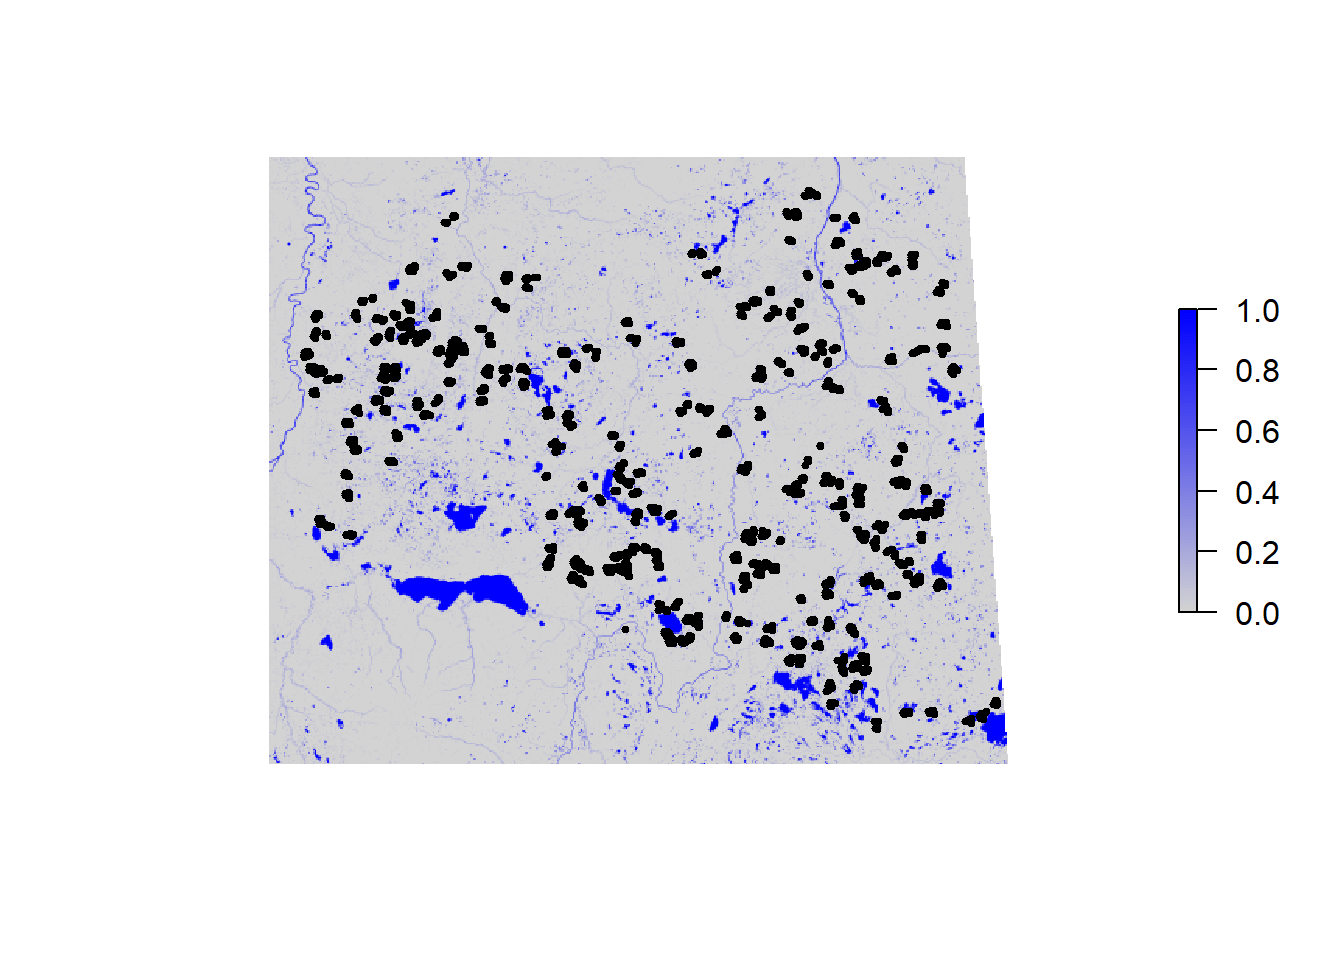
\includegraphics{qpad-book_files/figure-latex/data_xy-1.pdf}

\begin{Shaded}
\begin{Highlighting}[]
\NormalTok{cn <-}\StringTok{ }\KeywordTok{c}\NormalTok{(}\StringTok{"Open"}\NormalTok{, }\StringTok{"Water"}\NormalTok{, }\StringTok{"Agr"}\NormalTok{, }\StringTok{"UrbInd"}\NormalTok{, }\StringTok{"SoftLin"}\NormalTok{, }\StringTok{"Roads"}\NormalTok{, }
  \StringTok{"Decid"}\NormalTok{, }\StringTok{"OpenWet"}\NormalTok{, }\StringTok{"Conif"}\NormalTok{, }\StringTok{"ConifWet"}\NormalTok{)}
\CommentTok{#plot(x[,cn])}
\end{Highlighting}
\end{Shaded}

Add here:

\begin{itemize}
\tightlist
\item
  those kinds of transformations that are needed for regression
\item
  need to add absolute links to figures???
\end{itemize}

Exercise:

\begin{itemize}
\tightlist
\item
  play with the data to understand the distributions
\item
  use \texttt{summary}, \texttt{table}, \texttt{hist}, \texttt{plot}
\end{itemize}

\BeginKnitrBlock{rmdexercise}
This is an exercise.
\EndKnitrBlock{rmdexercise}

\BeginKnitrBlock{rmdnote}
This is a note.
\EndKnitrBlock{rmdnote}

\BeginKnitrBlock{rmdwarning}
This is a warning.
\EndKnitrBlock{rmdwarning}

\hypertarget{regression}{%
\chapter{A Primer in Regression Techniques}\label{regression}}

\begin{quote}
All models are wrong, but some are useful -- Box
\end{quote}

lm, glm

main effects, interactions, offsets

lasso, brt, boot/bagging, glmm

conditional and marginal effects

maybe opticut

cloglog motivation

\hypertarget{behavior}{%
\chapter{Behavioral Complexities}\label{behavior}}

Behaviour related stuff

constant p (time as covariate)

time varying p

finite mix

time varying p/c

rate, count, time-to-event

\hypertarget{detection}{%
\chapter{The Detection Process}\label{detection}}

EDR, tau constant

truncated, unlimited

variable tau: habitat effect (continuous case?)

discrete: land cover, observer effects

contrast fixed effects with offsets -- motivation for ARU

\hypertarget{recordings}{%
\chapter{Dealing with Recordings}\label{recordings}}

integration challenges

calibration (exponential/cloglog approximation)

fixed effects

paired

sensor sensitivity - EDR

\hypertarget{assumptions}{%
\chapter{A Closer Look at Assumptions}\label{assumptions}}

break thos assumptions

\hypertarget{roadsides}{%
\chapter{Understanding Roadside Surveys}\label{roadsides}}

directional diff in signal transmission

\hypertarget{extras}{%
\chapter{Miscellaneous Topics}\label{extras}}

model selection and conditional likelihood

variance/bias trade off

error propagation

MCMC?

N-mixture ideas

phylogenetic and life history/trait stuff

PIF methods

\bibliography{book.bib,packages.bib}


\end{document}
